\documentclass[11pt]{article} %Sets the default text size to 11pt and class to article.
\usepackage{amsmath}
\newcommand{\BigO}[1]{\ensuremath{\operatorname{O}\bigl(#1\bigr)}}
%------------------------Dimensions--------------------------------------------
\topmargin=-.5in %length of margin at the top of the page (1 inch added by default)
\oddsidemargin=-0.2in %length of margin on sides for odd pages
\evensidemargin=0in %length of margin on sides for even pages
\textwidth=6.5in %How wide you want your text to be
\marginparwidth=0.5in
\headheight=0pt %1in margins at top and bottom (1 inch is added to this value by default)
\headsep=0pt %Increase to increase white space in between headers and the top of the page
\textheight=10.0in %How tall the text body is allowed to be on each page
\pagestyle{empty}
\begin{document}
\centerline{{ \LARGE \bf Problem Set 8}} 
\centerline{CSCI 3104 $\bullet$ Spring 2014 $\bullet$ Birthday: 07/03} 
\centerline{Alexander Tsankov}
\line (1,0){470}
\\
\\
\noindent{\Large \bf Problem 1}
\\
\\
\noindent{ \large a) See Fig. 1 below. The minimum cut required for this graph would be to cut the edges emerging from "s". This requires only two cuts, and will cut a total of 17 capacity. This is the dotted line on Figure 1. 
\\
\begin{figure}[ht!]
\centering
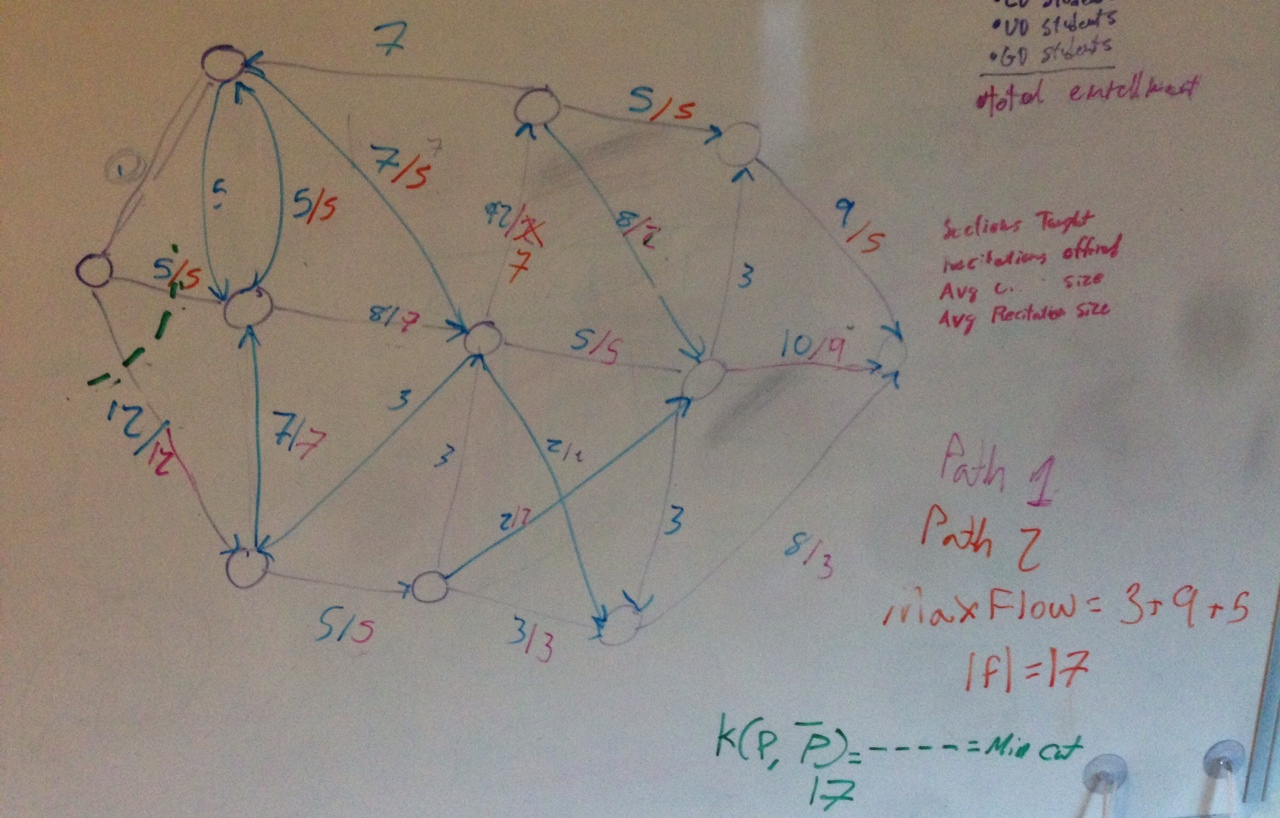
\includegraphics[width=120mm]{orig_flow.JPG}
\caption{Our original flow graph.}
\label{overflow}
\end{figure}
\\
\noindent{ \large b) The smallest capacity to increase water flow across the network would be 3. This is the maximum capacity that can be supported in terms of flow. See Fig. 2 below for our new network.} 
\\
\begin{figure}[ht!]
\centering
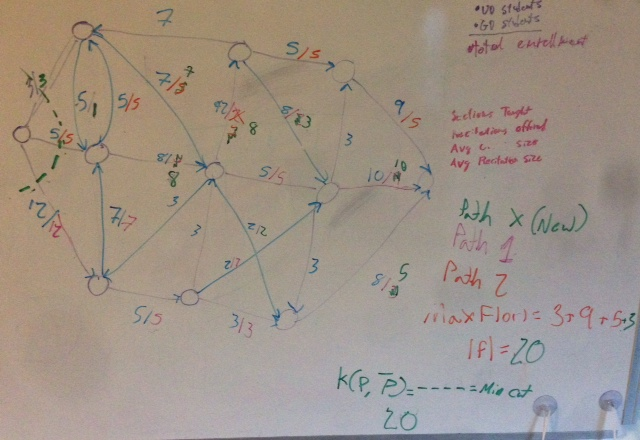
\includegraphics[width=110mm]{new_flow.JPG}
\caption{New modified flow graph with x = 3. }
\label{overflow}
\end{figure}
\\
\noindent{ \large c) The engineers can use the Ford-Fulkerson (FF) algorithm and the residual graph it produces to determine the max capacity of edge X. For problem B, we used the FF algorithm to discover that the maximum flow that can be pushed through X is 3. Anything beyond that can't be dealt with properly by the system and we get bottlenecking in the middle of the network. If we have graph G, the capacity of proposed Edge (u,v) is the max capacity of our our current graph ($M$) subtracted from the max capacity of our augmented graph ($M'$) i.e. $X = M' - M$ } 
\\
\\
\noindent{\Large \bf Problem 2}
\\
\noindent{\large a) See Fig. 2 for a visualization of the graph. If we take Path 1, our probability, $P_1$, of encountering a ringwraith is .96875. We reached this number by subtracting the combined likelihood of not encountering a ringwraith on Path 1, $(\frac{1}{2}*\frac{1}{2}*\frac{1}{2}*\frac{1}{2}*\frac{1}{2})$ or $.03125 $ from 1, which gives us a $P_1$ $= .96875$. The $P_2$ for Path 2 is simply $.97*1$, a .97 percent chance of encountering a ringwraith. Therefore, if we hope to minimize our probability for encountering a ringwraith, Path 1 would be better.
\\
\\
\noindent{\large However, if we calculate the expected value, $E_1$, of Path 1, which we can do by calculating probability of encountering a monster on each edge multiplied by 1, and eventually adding the total $(\frac{1}{2}*1 + \frac{1}{2}*1 + \frac{1}{2}*1 + \frac{1}{2}*1 + \frac{1}{2}*1),$ or $2.5$. The $E_2$ value of Path 2 is $(.97*1)$, or $.97$. The path with the lower $E$ is Path 2.   
\\
\\
\noindent{\large b) To find the path with the lowest possible expected value or $EV$ of encountering ringwraiths, we can use Dijkstra's algorithm (DA) on a modified graph. \\\\ Step 1) We begin by splitting every edge and creating a directed graph. We calculate the weight for these two new edges, for example (u,v) and (v,u) by taking the previous edge weight, (u,v), and adding it to the weight of the vertex $W(u,v) = P(u) + P(u,v)$ and $W(v,u) = P(v) + P(u,v)$ .  This takes $O(2E)$ time, two calculations for each newly-split edge. \\Step 2) Run DA on the modified paths to find the SSSP. This takes $O(E + V lg(V))$\\If we put together Step 1 and Step 2, we have a total run time of $O(E + V lg(V) + 2E)$  }
\\
\\
\noindent{\large c)To find the path with the lowest possible probability or $P$ of encountering  ringwraiths, we can use DA on a modified graph. \\\\ Step 1) We begin by splitting every edge and creating a directed graph. We calculate the weight for these two edges, in our case (u,v) and (v,u) by taking the previous edge weight and multiplying it by the negative logarithm of the probability of the vertex. For example, $W(u,v) = -log(P(u) * P(u,v))$ and $W(v,u) = log(P(v) * P(u,v)$. By using logarithms we avoid negative path weights that would break DA. This takes $O(2E)$ time, like the problem above. \\Step 2) Run DA on the modified paths to find the SSSP. This takes $O(E + V lg(V))$\\If we put together Step 1 and Step 2, we have a total run time of $O(E + V lg(V) + 2E)$}
\\
\\
\noindent{\Large \bf Problem 3}
\\
\indent{\large a) If we have a graph G with four vertices:\{A, B, C, D\}, with weighted edges:\{AB:1, AC:12, BC: 1, CD: 2\}, we will have a unique minimum spanning tree. This graph has the following two spanning trees from vertex A with edges: $T_1=$\{AB:1, BC:1, CD:2\} and $T_2=$\{AB:1,AC:12,CD:2\}. Even though there are two spanning trees, there is only one, unique MST ($T_1$).}
\\

\indent{\large b) For this problem, we must assume that edge weights do not have to be distinct. If all edge weights are distinct, then Golum would be correct. So, assuming we can have multiple edges with the same weight, the following undirected graph $G$ has two MSTs: \\vertices:\{A, B, C, D, E, F\}\\edges:\{AE:2, AB:4, BC:4, BD:4, DC:4, CF:2\} \\We can see that no edge is unique, and there is still two minimum spanning trees, therefore Golum's claim is incorrect.See Figure 3 for an illustration of this.}
\\
\\
\indent{\large c) For this claim, we must assume that edge weights do not have to be distinct. To prove the claim by contradiction we say that graph $G$ has two minimum spanning trees, $T_{MST}$ and $T'_{MST}$. Let edge $(u,v)$ be in the minimum spanning tree $T_{MST}$, but not $T'_{MST}$. If we were to remove the edge from $T_{MST}$, we will cut the tree into two partitions, $T_u$ and $T_v$. Next, let the edge $(a,b)$ be the unique minimum edge crossing the partition. Given $(x,y) \neq (u,v)$ and we know the weight of $(a,b)$$<$ the weight of $(u,v)$, therefore the spanning tree $(T_{MST}-(u,v))\cup(a,b)$ has a less weight than $T_{MST}$, which is a contradiction. Now, since the edge $(u,v)$ is not in $T'_{MST}$, we say that the path between $u$ and $v$ is path $l$.  Because path $l$ exists, we know that there is some edge, $e$, between $T'_u$ and $T'_v$ (A partition of $T'_{MST}$ where $u$ is in $T'_u$ and $v$ is  in$T'_v$). Now, we also know that $W(u,v)<W(e)$ because as stated above, $(u,v)$ is an unique minimum weighted edge. If we add $(u,v)$ to $T'_{MST}$ we get a cycle composed of the edge $(u,v)$ and the path $l$. By removing any edge from the cycle we get the
spanning tree $(T′_{MST} \cup (u,v)) − e$ which has a lower weight than $T′_{MST}$, this is also a contradiction. Therefore we know that given our claim, there can only be one, unique minimum spanning tree.}
\\
\indent{\large d) To do this, we will modify Kruskal's algorithm which takes $O(E*lg(V))$. We can take Kruskal's, and add some checks in the pseudo-code algorithm shown below, to confirm our analysis in part 3C: 
\begin{verbatim}
uniqueMST(G){ 
  int x[] = sortEdges(G) //array of sorted edges
  tree MST = initialize tree
  boolean uniqueCycle = false
  boolean uniqueMinPart = false
  for(i=1; i < x.length; i++){
    if(createsCycle(MST, x[i])){
      if(isMaxUniqueEdge(x[i]))
        uniqueCycle = true
    }
    else{
      addToTree(x[i])
      if(isMinEdgeConnectingPartitions(MST, x[i]))
        uniqueMinPart = true
    }
  }
  if(uniqueCycle && uniqueMinPart)
    return true
  else
    return false
}
\end{verbatim}
This algorithm performs Kruskal's algorithm, while checking to see if our claim from above is satisfied, thus returning true if there is only one, unique MST.
}
\\
\\
\noindent{\Large \bf Problem 4}
\\
\indent{\large To find a solution to solve this dilemma of uncooperative hobbits, we need to break it into two sub-problems. Problem a involves transforming our given graph into a flow diagram. Problem b requires us to run analysis on this flow to determine if it is possible for the hobbits to each reach the market while abiding by the rules given to us.}
\\
\indent(\large a) Because we know that the hobbits can never travel on the same path together, we can make each path have a maximum capacity of 1. This satisfies the requirement of only a single hobbit being on a path at once. We can see a transformation of a normal graph to our flow diagram in Figure 3 below. We know automatically for our new transformed graph that there has to be two paths out of $s$, and that there are two paths going to $t$. To find whether or not the paths in the middle are sufficient,we continue to part b, below. 
\\
\begin{figure}[ht!]
\centering
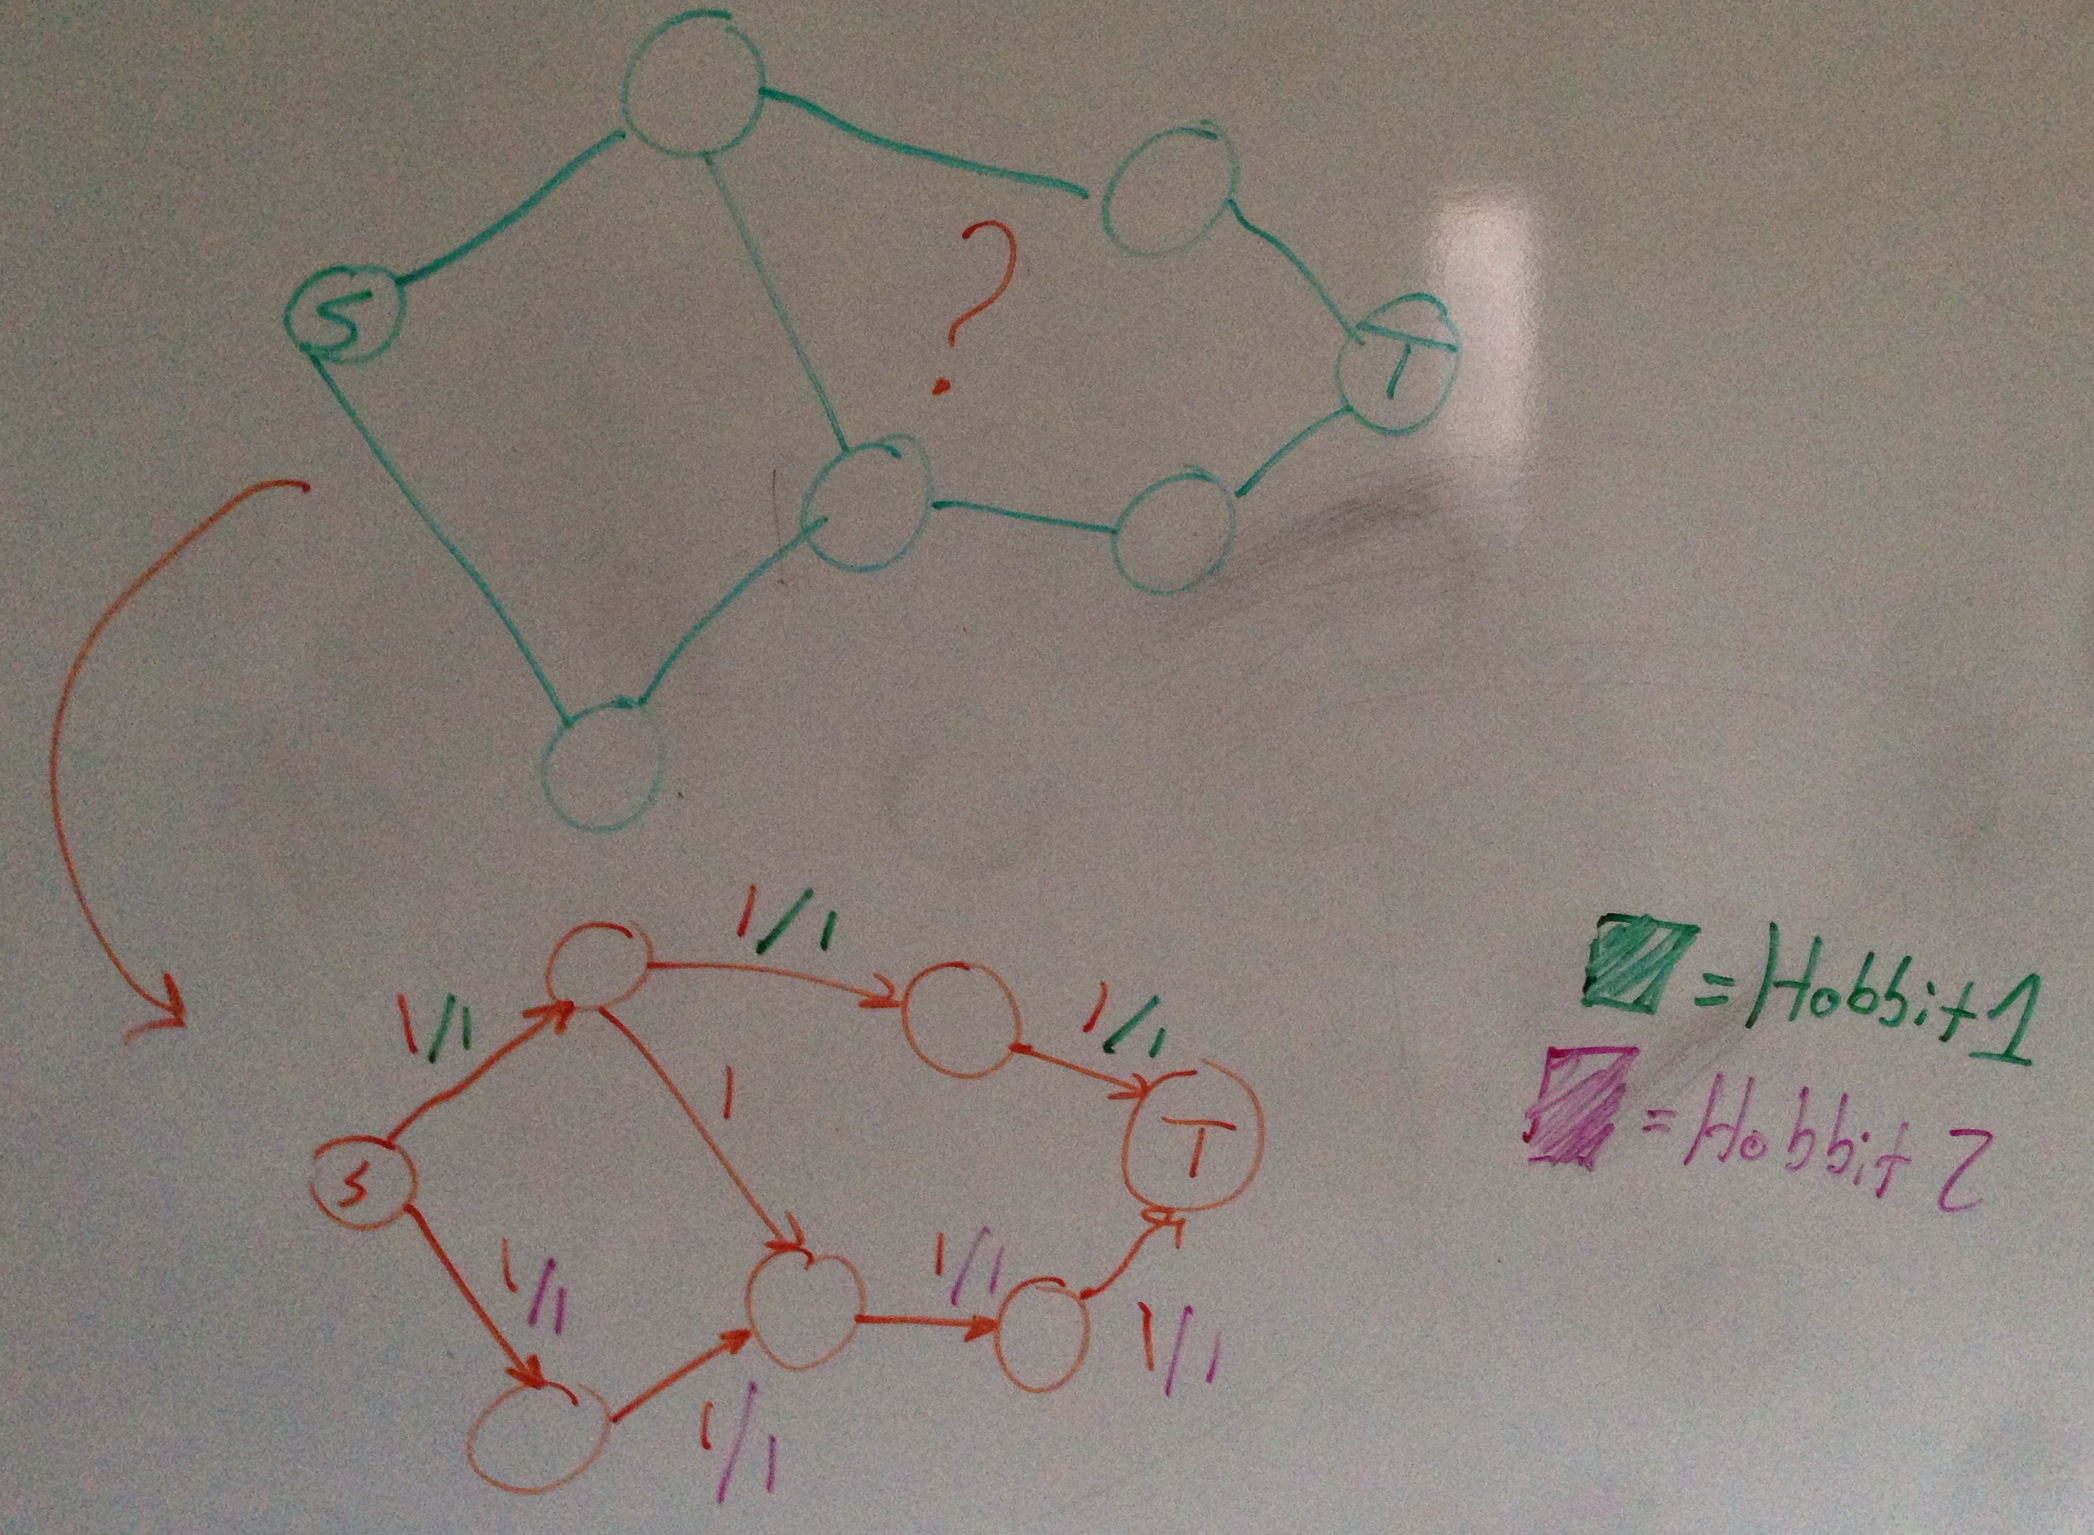
\includegraphics[width=110mm]{prob_4.JPG}
\caption{Transforming Graph and finding proper flow paths. }
\label{overflow}
\end{figure}
\\
\indent{\large b) Once we have our graph converted it is simply a matter of running the Ford-Fulkerson algorithm for max-flow to find the proper path for the hobbits to take given the restrictions. Look at Figure 3 to see how we ran the FF algorithm on our two flows to find the possible paths for the hobbits. 
\\
\\
\noindent{\Large \bf Problem 5}
\\
\indent{\large To solve the poisoned wine problem, we need to give each of the bottles a serial number in binary. Bottle 1 (B1) would be given the label (1), Bottle 2 would have the label (10) with Bottle 11 having the label (1011), etc. Each rat is labelled with a bit, and they only sip from the wine that uses their bit. So in the case Rat 1, he only drinks from wines with the first bit activated (1001,0011,101,...1). Rat 2, attached to the second bit, will only drink from bottles with the second bit activated (11,101010, 11010,...). If, in our case, a bottle is poisoned, we can see the chain of rats with each dead rat representing a bit of our poisoned bottle's serial number. If rats 1,2,4 die, we know that the number of our bad bottle is (1011) or Bottle 11. For n bottles, we need O$(lg(n))$ rats. See the table below for a sample of 4 rats with 15 bottles of wine, including a poisoned bottle 6. By finding that Rats 2,3 are dead, we know that bottle (0110) is poisoned. This is the bottle 6 that we expected. 
\\ 
\centerline{\begin{tabular}{ l | c | r }
  \hline                       
  Rat (Bit) & Bottles Consumed & Dead \\\hline
  1(0001) & 1,3,5,7,9,11,13,15 & N \\
  2(0010) & 2,3,6,7,10,11,14,15 & Y \\
  3(0100) & 4,5,6,7,12,13,14,15 & Y \\
  4(1000) & 8,9,10,11,12,13,14,15 & N \\
  \hline  
\end{tabular}}
\\
\newline
\noindent{ \Large \bf Sources}
\\
\noindent{$\bullet$ https://www.cs.princeton.edu/courses/archive/spring13/cos423/lectures/07NetworkFlowI-2x2.pdf}
%USEFUL FOR FLOWS%
\\
\noindent{$\bullet$ http://en.wikipedia.org/wiki/Bellman%E2%80%93Ford_algorithm#Algorithm}
\\
\noindent{$\bullet$ http://math.stackexchange.com/questions/94414/an-algorithm-for-arbitrage-in-currency-exchange}
\\
\noindent{$\bullet$http://code.activestate.com/recipes/119466-dijkstras-algorithm-for-shortest-paths/}
\\
\end{document}